\input templates/header
\title[DS - BFT]{\textbf{Distributed Algorithms}\\Practical Byzantine Fault Tolerance}

\graphicspath{{figs/16/}}

\newcommand{\Retreat}{\textsc{retreat}}

\newcommand{\OM}{\textit{OM}}


\newcommand{\Request}{\textsc{request}}
\newcommand{\Preprepare}{\textsc{pre-prepare}}
\newcommand{\Prepare}{\textsc{prepare}}
\newcommand{\Commit}{\textsc{commit}}
\newcommand{\Reply}{\textsc{reply}}
\newcommand{\Checkpoint}{\textsc{checkpoint}}
\newcommand{\ViewChange}{\textsc{view-change}}
\newcommand{\NewView}{\textsc{new-view}}

\newcommand{\Prepared}{\mathbf{prepared}}
\newcommand{\Committed}{\mathbf{committed}}




\begin{document}


\FrameTitle{}
\FrameContent


%%%%%%%%%%%%%%%%%%%%%%%%%%%%%%%%%%%%%%%%%%%%%%%%%%%%%%%%%%%%%%%%%%%%%%%%%%
\section{Introduction}


%-------------------------------------------------------------------------
\begin{frame}{Motivation}

\BI
\item Processes may exhibit arbitrary (Byzantine) behavior
	\BI
	\item Malicious attacks
		\BI
		\item They lie
		\item They collude
		\EI
	\item Software error
		\BI
		\item Arbitrary states, messages
		\EI
	\EI
\EI
	
\begin{block}{Examples}
\BI
\item Amazon outage (2008), “Root cause was a single bit flip in internal state messages”\footnotemark
\item Shuttle Mission STS-124 (2008), 3-1 disagreement on sensors during fuel loading (on Earth!)\footnotemark
\EI
\end{block}
\footnotetext{\url{http://status.aws.amazon.com/s3-20080720.html}}
\footnotetext{\url{https://c3.nasa.gov/dashlink/resources/624/}}

\end{frame}


%-------------------------------------------------------------------------
\begin{frame}{History}

\BIL
\item State-of-the-art at the end of the 90's
\BI
\item Theoretically feasible algorithms to tolerate Byzantine failures, but inefficient in practice
\item Assume synchrony – known bounds for message delays and processing speed
\item Most importantly: synchrony assumption needed for correctness – what about DoS?
\EI
\EIL

\bigskip
\begin{Bib}
	\bibentry{byzgenerals}
\end{Bib}

\end{frame}

\section{Byzantine generals}

%-------------------------------------------------------------------------
\begin{frame}{Byzantine generals}
	
\begin{figure}
	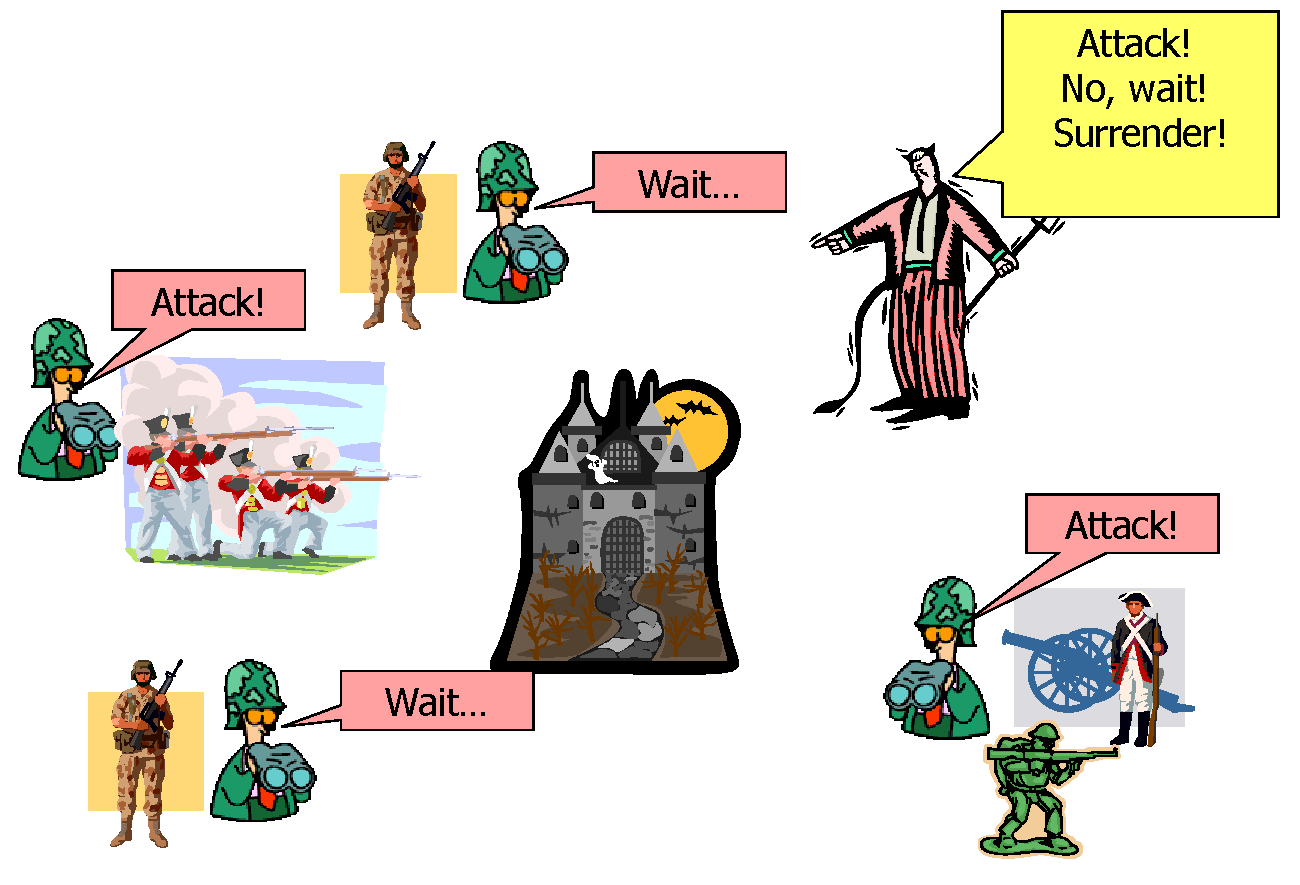
\includegraphics[width=0.9\textwidth]{generals}
\end{figure}

\end{frame}

%-------------------------------------------------------------------------
\begin{frame}{Specification}

\BIL
\item A \alert{commanding general} must send an order to his $n-1$ \alert{lieutenant generals} such that:
\BI
\item \textbf{IC1}: All loyal lieutenants obey the same order
\item \textbf{IC2}: If the commanding general is loyal, then every loyal lieutenant obeys the order he sends
\EI
\item Assumptions (“Oral” messages):
\BI
\item Every message that is sent is received correctly
\item The receiver of a message knows who sent it
\item The absence of a message can be detected
\EI
\EIL

\end{frame}

%-------------------------------------------------------------------------

\begin{frame}{Impossibility results}
	
Under the “Oral” messages assumption, no solution with three generals can handle even 
a single traitor
	
\begin{figure}
	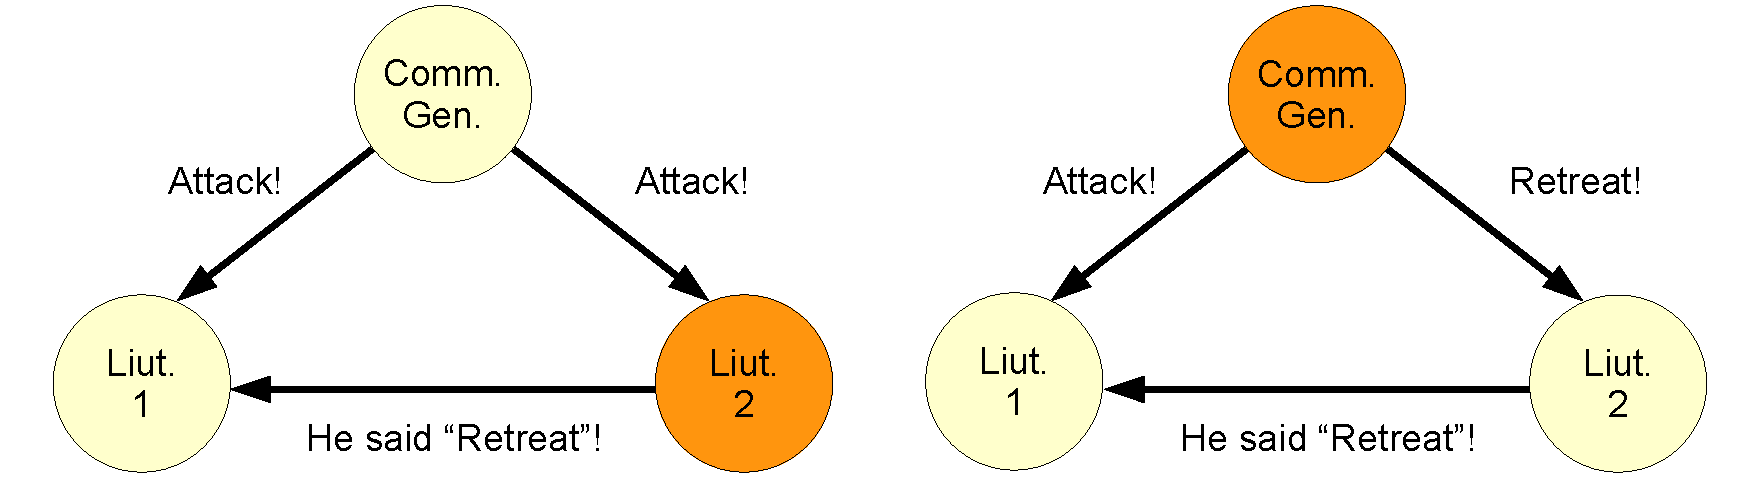
\includegraphics[width=\textwidth]{impossibility}
\end{figure}

\end{frame}


%-------------------------------------------------------------------------
\begin{frame}{“Oral Message” algorithm $\OM(m)$}

\BIL
\item Algorithm $\OM(0)$
	\BE
	\item The commander sends its value to every lieutenant
	\item Each lieutenant uses the value he received from commander, or uses $\Retreat$ if he received no value
	\EE
\item Algorithm $\OM(m)$
	\BE
	\item The commander send its value to every lieutenant
	\item $\forall i$, let $v_i$ be the value lieutenant $i$ receives from the
	commander, or $\Retreat$ if it has received no value. Lieutenant $i$ acts as the
	commander of algorithm $\OM(m-1)$ to send the value $v_i$ to each of the other $n-2$
	other lieutenants
	\item $\forall j \neq i$, let $v_j$ be the value received by $i$ from $j$
	in Step 2 of algorithm $\OM(m-1)$ or $\Retreat$ if no value. Lieutenant $i$ uses
	the value $\mathsf{majority}(v_1, ..., v_n)$ (deterministic function)
	\EE
\EIL

The recursive
\end{frame}

\begin{frame}{“Oral Message” Algorithm Example -- $\OM(1)$}
	
\begin{figure}	
	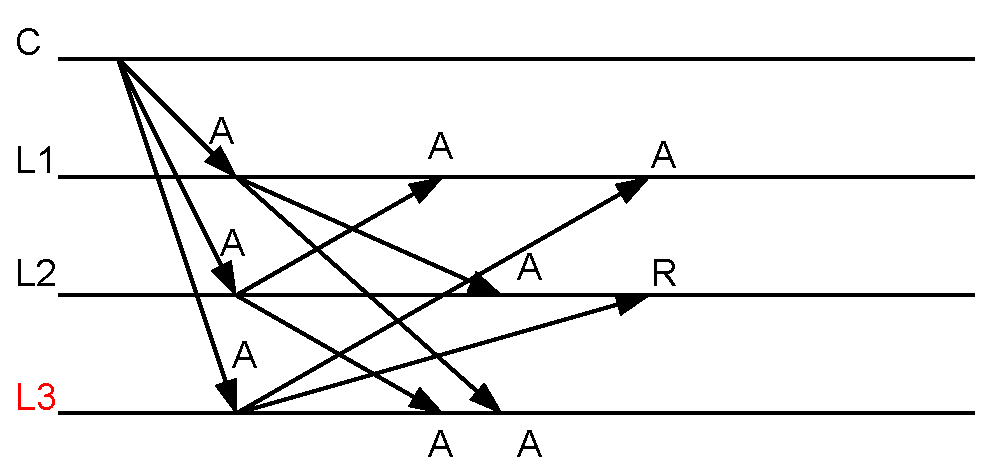
\includegraphics[width=\textwidth]{oral}
\end{figure}
	
\end{frame}



%-------------------------------------------------------------------------
\begin{frame}{Oral messages}
	
\begin{theorem}
For any $m$, Algorithm $\OM(m)$ satisfies conditions \textbf{IC1} and \textbf{IC2} if there are more than $3m$ generals and at most $m$ traitors
\end{theorem}

\bigskip
\BIL
\item Problems:
\BI
\item message paths of length up to $m+1$  (expensive)
\item absence of messages must be detected via time-out\\ (vulnerable to DoS)	
\EI
\EIL

\note{

An attacker may compromise the safety of a service by delaying non-faulty
nodes or the communication between them until they are tagged as faulty and
excluded from the replica group. Such a denial-of-service attack is generally
easier than gaining control over a non-faulty node.

}

\end{frame}

%-------------------------------------------------------------------------
\section{Practical Byzantine Fault Tolerance}

\begin{frame}{A Byzantine “renaissance”}
		
\begin{Bib}
\bibentry{pbft-tocs}
\end{Bib}	

\smallskip
\structure{Contributions}
\BIL
\item First state machine replication protocol that survives Byzantine faults in asynchronous networks
\item Live under weak Byzantine assumptions – Byzantine paxos!
\item Implementation of a Byzantine, fault tolerant distributed FS
\item Experiments measuring cost of replication technique
\EIL
		
\end{frame}

%-------------------------------------------------------------------------
\begin{frame}{Assumptions}
\BIL
\item System model
	\BI
	\item Asynchronous distributed system with $N$ processes
	\item Unreliable channels
	\EI
\item Unbreakable cryptography
	\BI
	\item Message $m$ is signed by its sender $i$, and we write $\langle m \rangle_{\sigma(i)}$, through:
		\BI
		\item Public/private key pairs 
		\item Message authentication codes (MAC)
		\EI
	\item A digest $d(m)$ of message $m$ is produced through collision-resistant hash functions
	\EI
\EIL
\end{frame}

\note{MACs (message authentication codes) are based on secret keys (client-server, server-server)}

%-------------------------------------------------------------------------
\begin{frame}{Assumptions}
\BIL

\item Failure model
\BI
\item Up to $f$ Byzantine servers
\item $N > 3f$ total servers
\item (Potentially Byzantine clients)
\EI
\item Independent failures
\BI
\item  Different implementations of the service
\item Different operating systems
\item Different root passwords, different administrator
\EI

\EIL

\end{frame}


%-------------------------------------------------------------------------
\begin{frame}{Specification}

\BIL
\item State machine replication
\BI
\item Replicated service with a state and deterministic operations operating on it
\item Clients issue a request and block waiting for reply
\EI
\item Safety
\BI
\item The system satisfies linearizability, provided that $N>3f+1$
\item Regardless of “faulty clients”... 
	\BI
	\item all operations performed by faulty clients are observed in a consistent way by non-faulty clients
	\EI
\item The algorithm does not rely on synchrony to provide safety...
\EI
\item Liveness
\BI
\item It relies on synchrony to provide liveness
\item Assumes $\mathit{delay}(t)$ does not grow faster than $t$ indefinitely
\item Weak assumption – if network faults are eventually repaired
\item Circumvent the impossibility results of FLP
\EI
\EIL
\end{frame}


%-------------------------------------------------------------------------
\begin{frame}{Optimality}
	
\begin{theorem}
To tolerate up to $f$ malicious nodes, $N$ must be equal to $3f+1$
\end{theorem}
	
\bigskip
\begin{proof}
\BIL
\pause
\item It must be possible to proceed after communicating with $N-f$ replicas,
because the faulty replicas may not respond
\pause
\item But the $f$ replicas not responding may be just slow, so $f$ of those
that responded might be faulty
\pause
\item The correct replicas who responded ($N-2f$) must outnumber 
the faulty replicas, so
\[
  N-2f > f \Rightarrow N > 3f
\]
\EIL
\end{proof}
		
\end{frame}

%-------------------------------------------------------------------------
\begin{frame}{Optimality}
\BIL
\item So, $N>3f$ to ensure that at least a correct replica is present in the reply set
\item $N=3f+1$; more is useless
\BI
\item more and larger messages
\item without improving resiliency
\EI
\EIL
	
\end{frame}


%-------------------------------------------------------------------------
\begin{frame}{Processes and views}

\BIL
\item Replicas IDs: $0 \ldots N-1$
\item Replicas move through a sequence of configurations called \alert{views}
\item During view $v$:
\BI
\item \alert{Primary} replica is $i$: $i = v \bmod N$
\item The other are \alert{backups}
\EI
\item \alert{View changes} are carried out when the primary appears to have failed
\EIL	
	
\end{frame}

%-------------------------------------------------------------------------
\begin{frame}{The algorithm}
	
\begin{columns}
\begin{column}{0.6\textwidth}
\BI
\item To invoke an operation, the client sends a request to the primary
\item The primary multicasts the request to the backups
\item Quorums are employed to guarantee ordering on operations
\item When an order has been agreed, replicas execute the request and send a reply to the client
\item When the client receives at least $f+1$ identical replies, it is satisfied
\EI
\end{column}
\begin{column}{0.4\textwidth}
	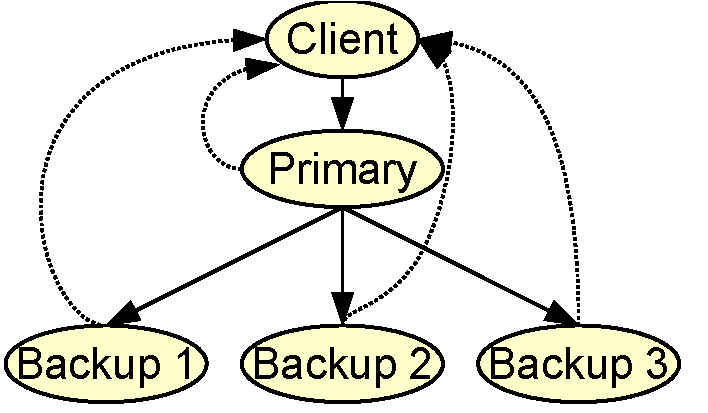
\includegraphics[width=\textwidth]{primary-backup}
\end{column}

\end{columns}	
	
\end{frame}


%-------------------------------------------------------------------------
\begin{frame}{Problems}

\BIL
\item \alert{The primary could be faulty!}
	\BI
	\item could ignore commands; assign same sequence number to different requests; skip sequence numbers; etc
	\item backups monitor primary's behavior and trigger view changes to replace faulty primary
	\EI
\item \alert{Backups could be faulty!}
	\BI
	\item could incorrectly store commands forwarded by a correct primary
	\item use dissemination Byzantine quorum systems
	\EI
\item \alert{Faulty replicas could incorrectly respond to the client!}
	\BI
	\item Client waits for $f+1$ matching replies before accepting response
	\EI
\EIL

\end{frame}

%-------------------------------------------------------------------------
\begin{frame}{The general idea}

\BIL
\item Algorithm steps are justified by \alert{certificates}
	\BI
	\item Sets (quorums) of signed messages from distinct replicas proving 
	that a property of interest holds
	\EI
\item With quorums of size at least $2f+1$
	\BI
	\item Any two quorums intersect in at least one correct replica
	\item There is always one quorum that contains only non-faulty replicas
	\EI
\EIL	

\begin{overprint}
\onslide<1|handout:1>
\begin{figure}
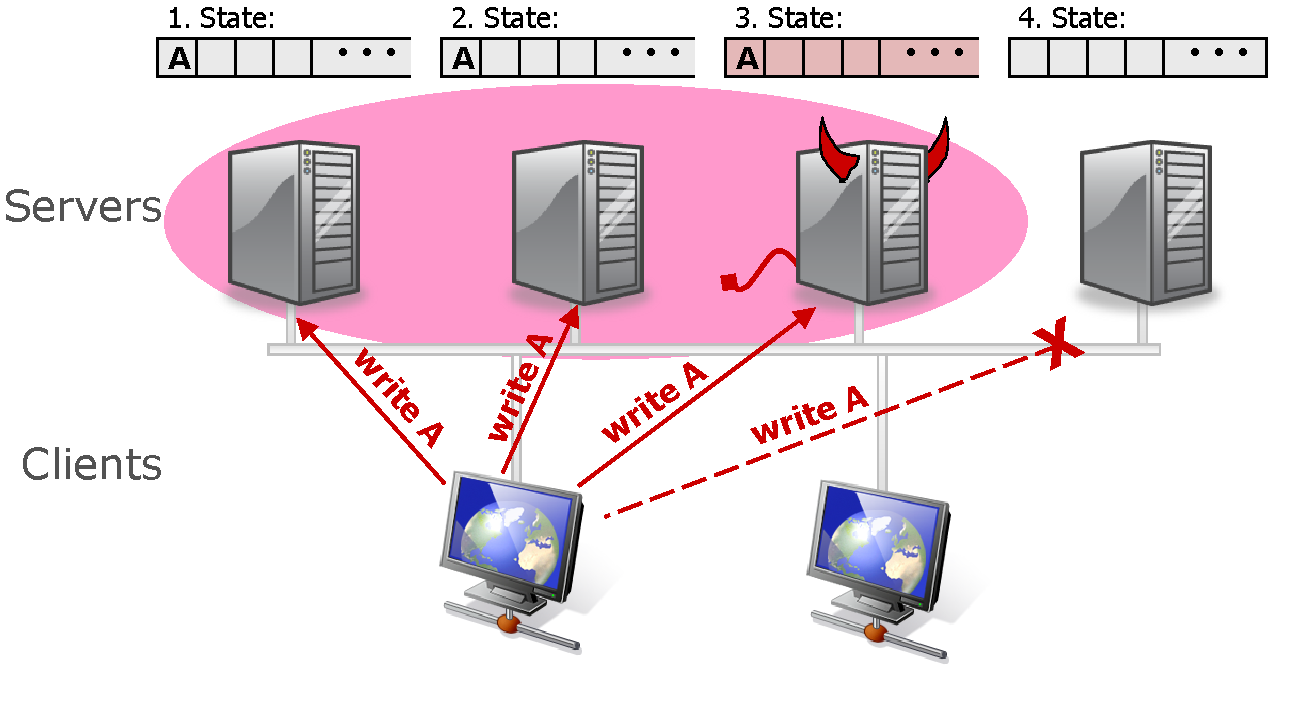
\includegraphics[width=0.7\textwidth]{quorum1}
\end{figure}
\onslide<2|handout:2>
\begin{figure}
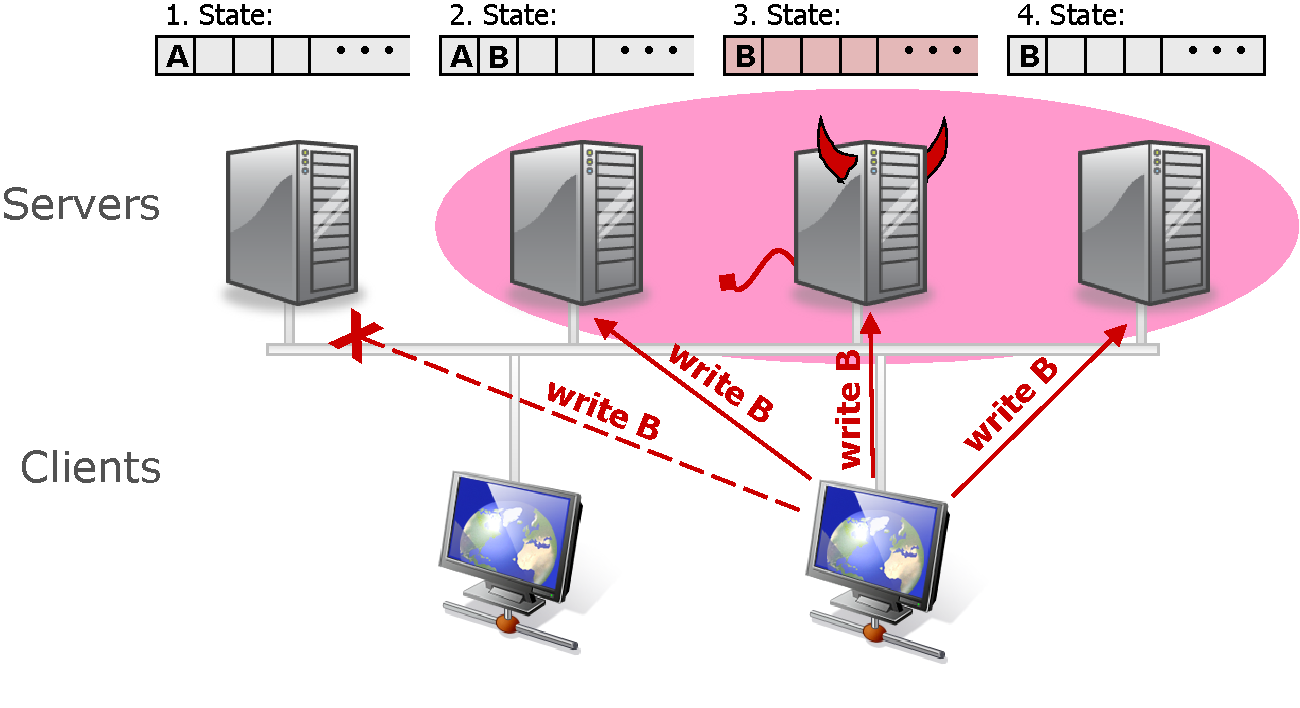
\includegraphics[width=0.7\textwidth]{quorum2}
\end{figure}
\end{overprint}
\end{frame}

%-------------------------------------------------------------------------
\begin{frame}{Protocol schema}
	
\BIL
\item Normal operation
	\BI
	\item How the protocol works in the absence of failures
	\item hopefully, the common case
	\EI
\item View changes
	\BI
	\item How to depose a faulty primary and elect a new one
	\EI
\item Garbage collection
	\BI
	\item How to reclaim the storage used to keep certificates
	\EI
\item Recovery
	\BI
	\item How to make a faulty replica behave correctly again (not here)	
	\EI
\EIL
\end{frame}

%-------------------------------------------------------------------------
\begin{frame}{State}
	
\BIL
\item The internal state of each of the replicas include:
\BI
\item the state of the actual service
\item a message log containing all the messages the replica has accepted
\item an integer denoting the replica current view
\EI
\EIL		
	
\end{frame}

%-------------------------------------------------------------------------
\begin{frame}{Client request}

\begin{figure}
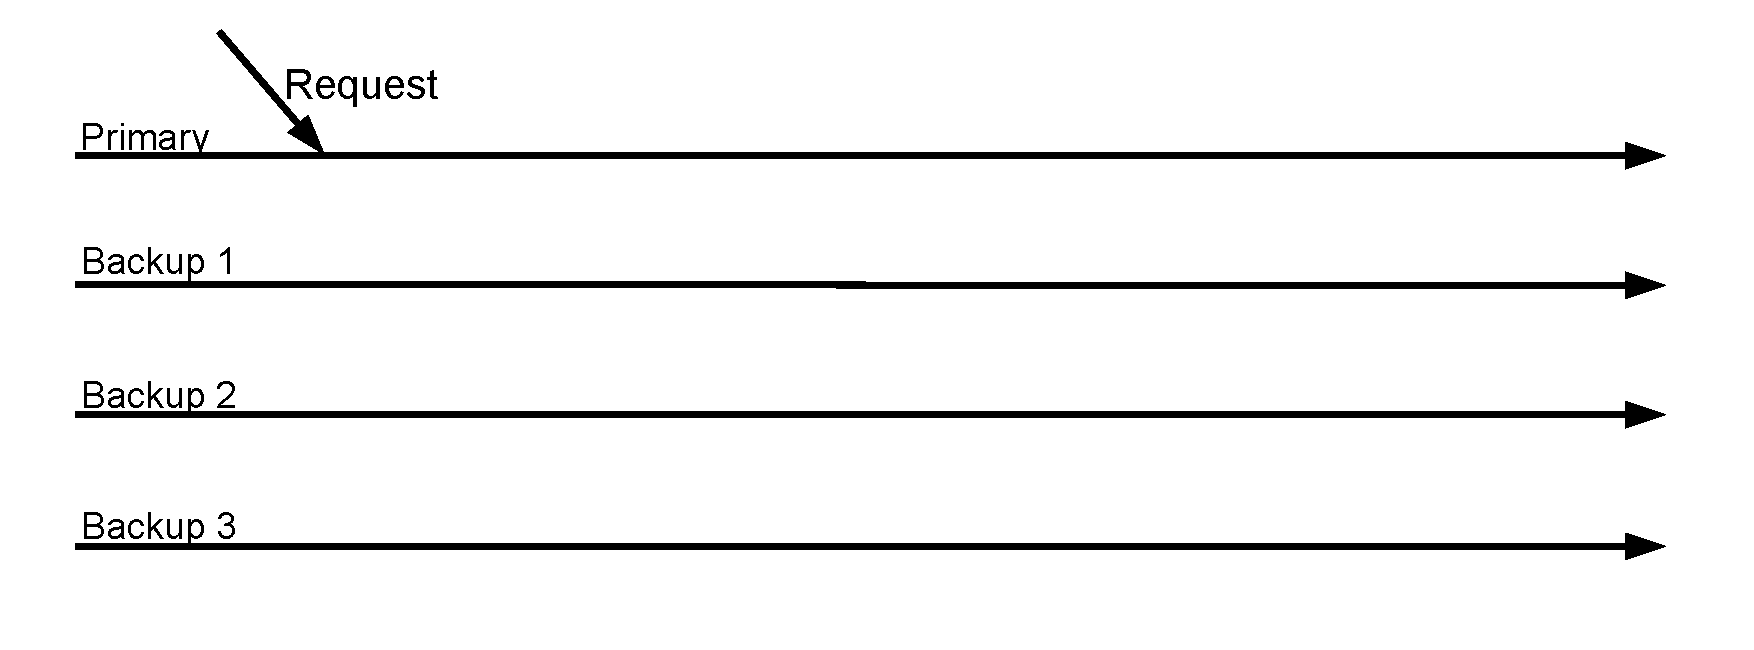
\includegraphics[width=0.9\textwidth, trim=0 20 0 60]{messages0}
\end{figure}
\structure{$\langle \Request, o, t, c \rangle_{\sigma(c)}$}
\BI
\item $o$: state machine operation
\item $t$: timestamp (used to ensure exactly-once semantics)
\item $c$: client id
\item $\sigma(c)$: client signature
\EI

\end{frame}

%-------------------------------------------------------------------------
\begin{frame}{Pre-prepare phase}

\begin{figure}
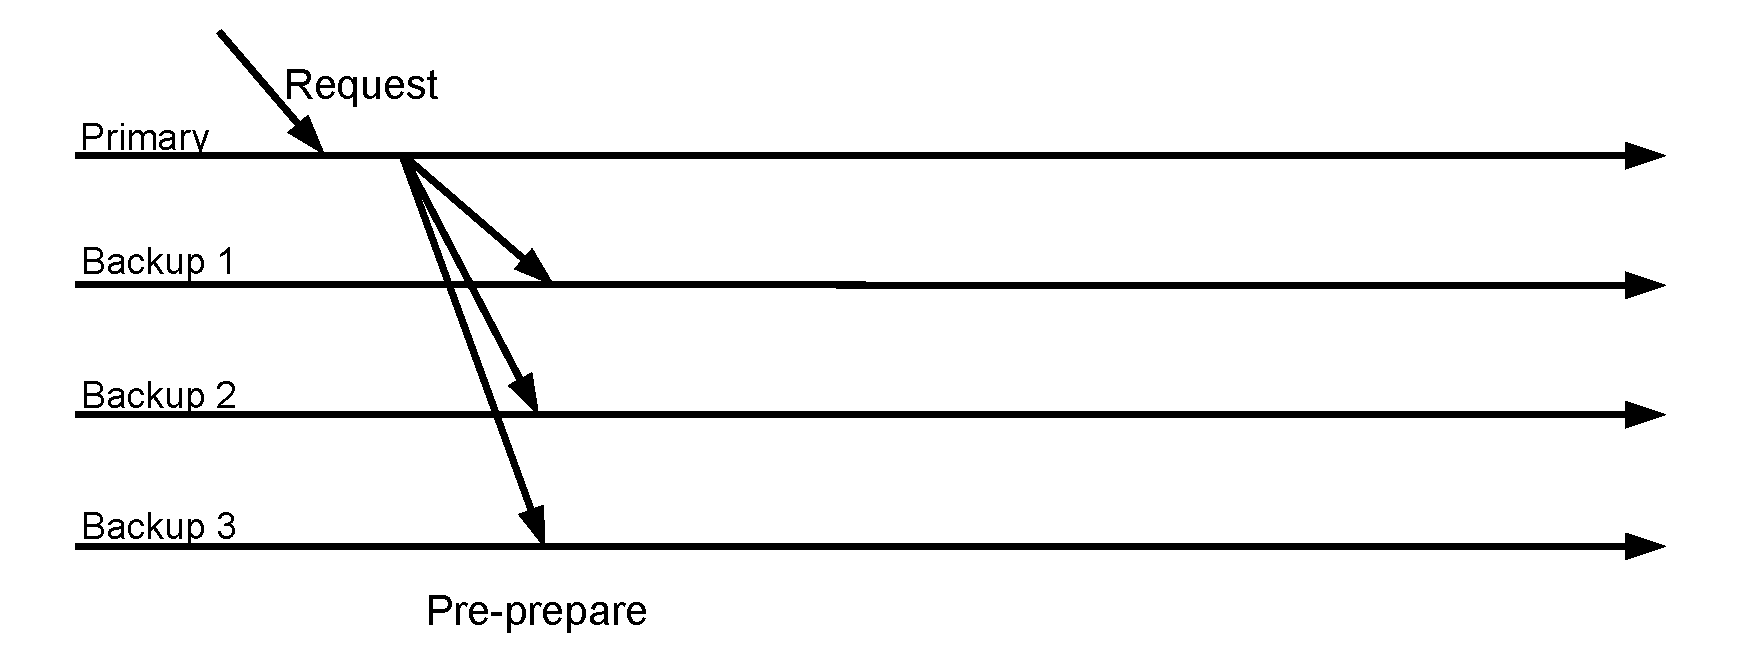
\includegraphics[width=0.9\textwidth, trim=0 20 0 60]{messages1}
\end{figure}
\structure{$\langle \langle \Preprepare, v, n, d(m) \rangle_{\sigma(p)}, m \rangle$}
\begin{columns}
	\begin{column}{0.5\textwidth}
	\BI
	\item $v$: current view
	\item $n$: sequence number
	\item $d(m)$: digest of client message
	\EI
	\end{column}
	\begin{column}{0.5\textwidth}
	\BI
	\item $\sigma(p)$: primary signature
	\item $m$: client message
	\EI
	\end{column}
\end{columns}

\note{
Requests are not included in pre-prepare messages to keep them small. This is
important because pre-prepare messages are used as a proof that the request
was assigned sequence number in view in view changes.
}


\end{frame}


%-------------------------------------------------------------------------
\begin{frame}{Pre-prepare phase}

\structure{$\langle \langle \Preprepare, v, n, d(m) \rangle_{\sigma(p)}, m \rangle$}
\BIL
\item  Correct replica $i$ accepts $\Preprepare$ if:
\BI
	\item the $\Preprepare$ message is well-formed
	\item the current view of $i$ is $v$
	\item $i$ has not accepted another $\Preprepare$ for $v, n$ with a different digest
	\item $n$ is between two water-marks $L$ and $H$\\
			(to avoid sequence number exhaustion caused by faulty primaries)
	\EI
\item Each accepted $\Preprepare$ message is stored in the
accepting replica's message log (including the primary's)
\item Non-accepted $\Preprepare$ messages are just discarded
\EIL

\end{frame}

%-------------------------------------------------------------------------
\begin{frame}{Prepare phase}

\begin{figure}
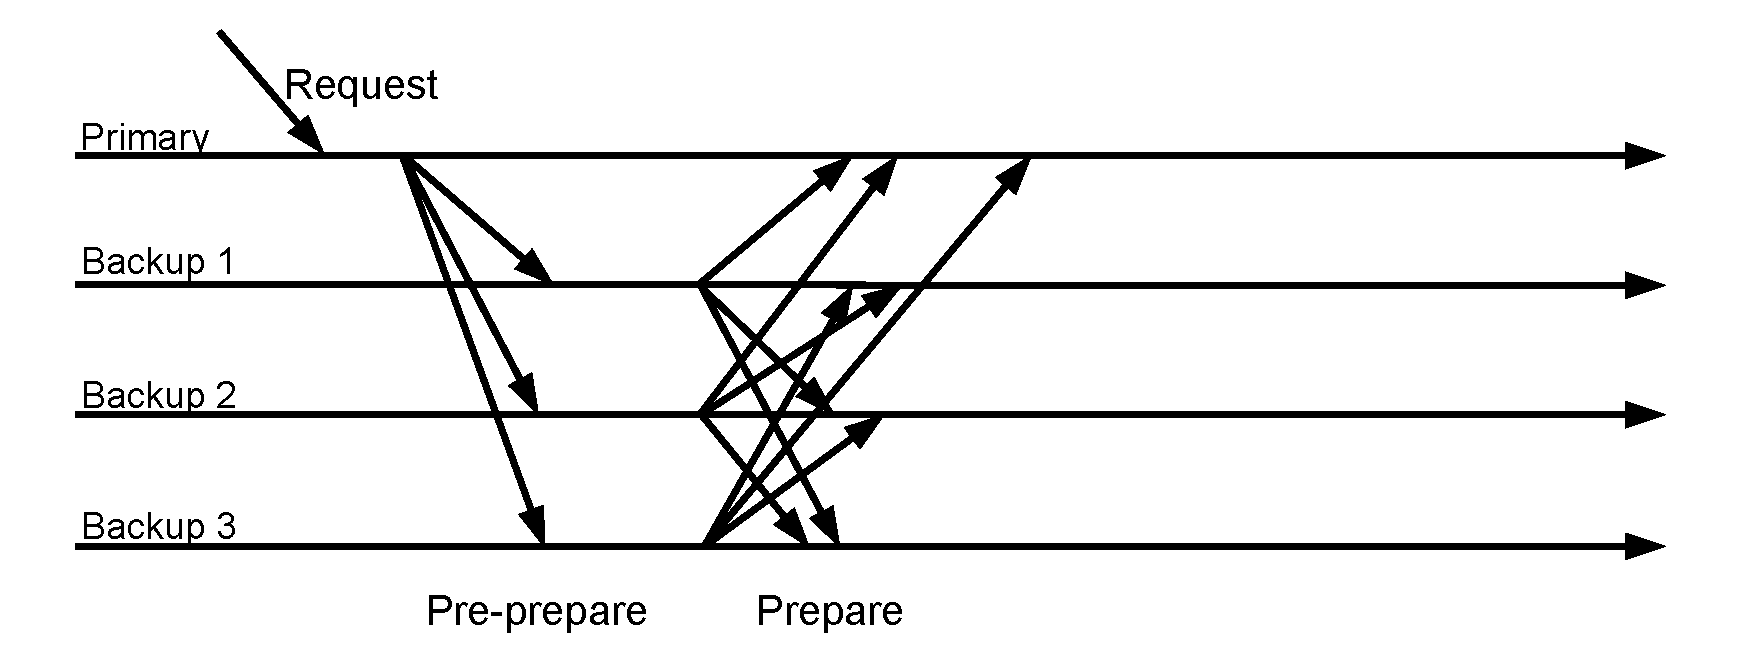
\includegraphics[width=0.9\textwidth, trim=0 20 0 60]{messages2}
\end{figure}
\structure{$\langle \Prepare, v, n, d(m) \rangle_{\sigma(i)}$}
\begin{overprint}
\onslide<1|handout:1>
\BI
\item Accepted by correct replica $j$ if:
\BI
\item the $\Prepare$ message is well-formed
\item current view of $j$ is $v$
\item $n$ is between two water-marks $L$ and $H$
\EI
\EI

\onslide<2|handout:2>
\BI
\item Replicas that send $\Prepare$ accept the sequence number $n$ for $m$ in view $v$
\item Each accepted $\Prepare$ message is stored in the accepting replica's message log
\EI

\end{overprint}
\end{frame}

%-------------------------------------------------------------------------
\begin{frame}{Prepare certificate (P-certificate)}

\BIL
\item Replica $i$ produces a \alert{prepare certificate} $\Prepared(m,v,n,i)$ iff its log holds:
	\BI
	\item The request $m$
	\item A $\Preprepare$ for $m$ in view $v$ with sequence number $n$
	\item Log contains $2f$ $\Prepare$ messages from different backups that match the $\Preprepare$
	\EI
\item $\Prepared(m,v,n,i)$ means that a quorum of \alert{$(2f+1)$} replicas agrees with assigning sequence number $n$ to $m$ in view $v$
\EIL

\smallskip
\begin{theorem}
There are no two non-faulty replicas $i, j$ such that $\Prepared(m, v, n, i)$
and $\Prepared(m',v , n, j)$, with $m \neq m'$
\end{theorem}

\smallskip
Proof?

\end{frame}

%-------------------------------------------------------------------------
\begin{frame}{Commit phase}
	
\begin{figure}
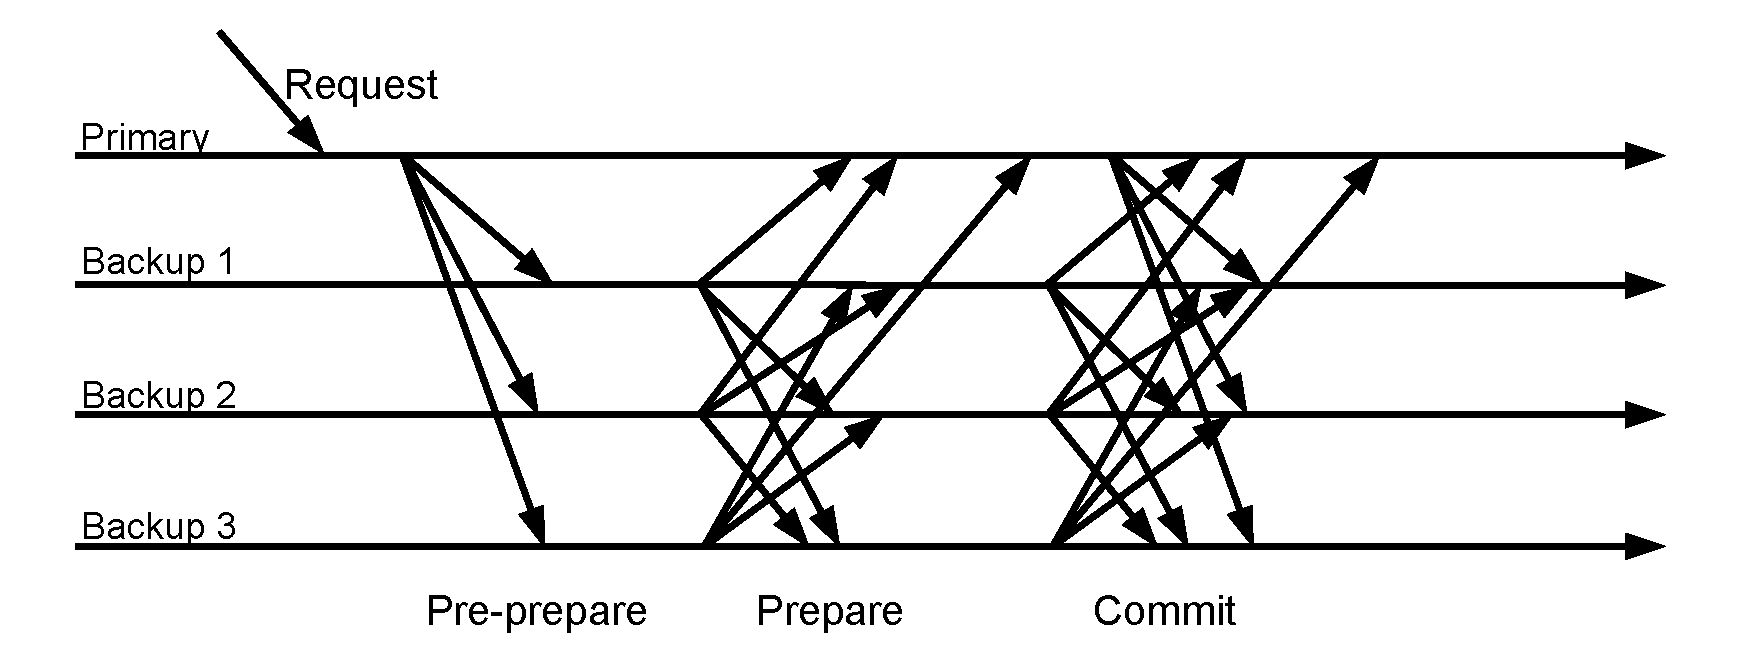
\includegraphics[width=0.9\textwidth, trim=0 20 0 60]{messages3}
\end{figure}
\structure{$\langle \Commit, v, n, d(m), i \rangle_{\sigma(i)}$}
\BIL
\item After having collected a P-certificate $\Prepared(m,v,n,i)$, replica $i$ sends a $\Commit$ message
\item Accepted if:
\BI
\item The $\Commit$ message is well-formed
\item Current view of $i$ is $v$
\item $n$ is between two water-marks $L$ and $H$
\EI
\EIL

\end{frame}

%-------------------------------------------------------------------------
\begin{frame}{Commit certificate (C-Certificate)}
	
\BIL
\item \alert{Commit certificates} ensure total order across views
	\BI
	\item we guarantee that we can't miss prepare certificates  during a view change
	\EI
\item A replica has a certificate $\Committed(m,v,n,i)$ if:
\BI
\item it had a P-certificate $\Prepared(m,v,n,i)$
\item log contains $2f +1$ matching $\Commit$ from different replicas (possibly including its own)
\EI
\item Replica executes a request after it gets commit certificate for it, and has cleared all requests with smaller sequence numbers
\EIL
\end{frame}

%-------------------------------------------------------------------------
\begin{frame}{Reply phase}
	
\begin{figure}
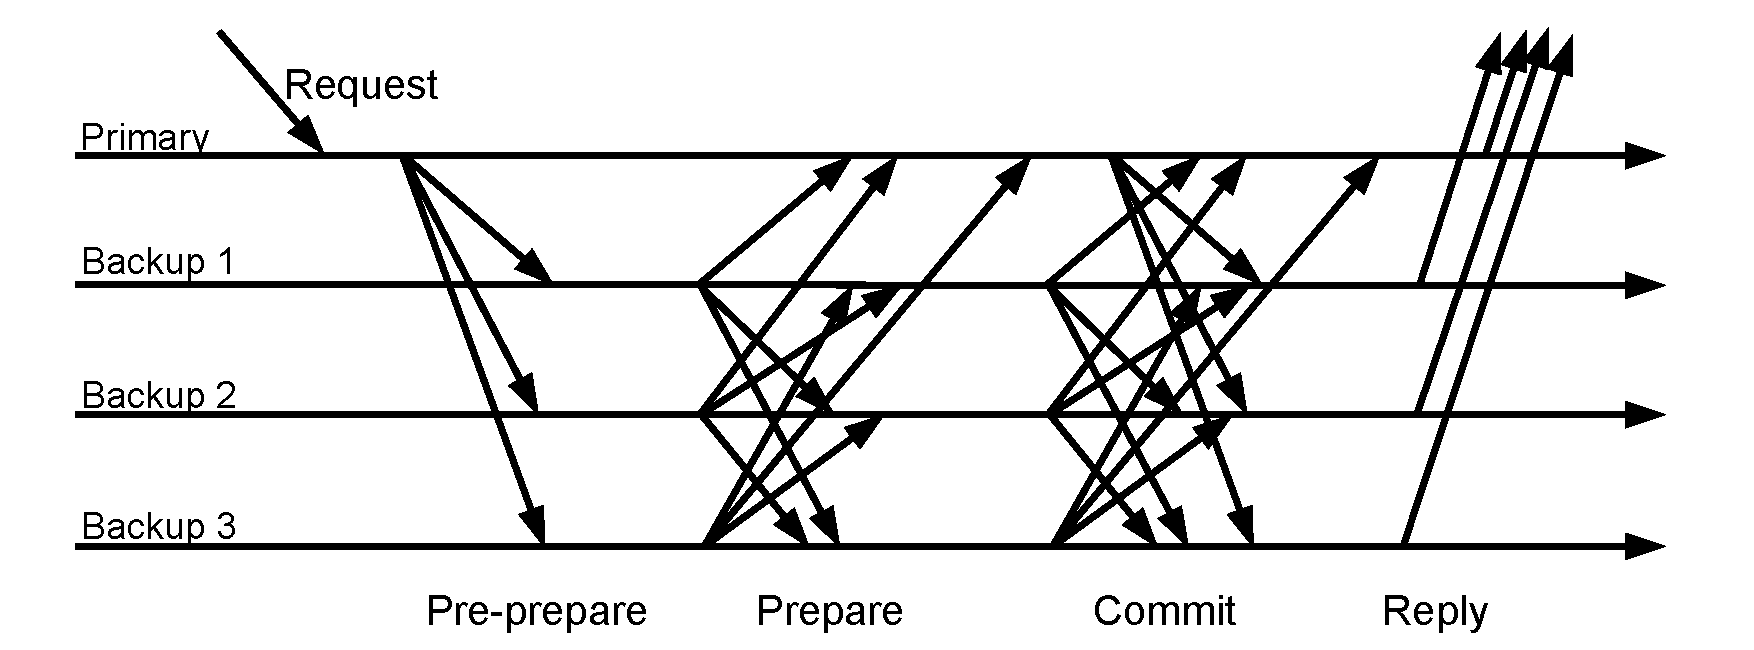
\includegraphics[width=0.9\textwidth, trim=0 20 0 60]{messages4}
\end{figure}
\structure{$\langle \Reply, v, t, c, i, r \rangle_{\sigma(i)}$}
\BIL
\item $r$ is the reply
\item Client waits for $f+1$ replies with the same $t,r$
\item If the client does not receive replies soon enough, it broadcast the request to all replicas
\EIL

\end{frame}

%-------------------------------------------------------------------------
\begin{frame}{View change}
	
\BIL
\item A un-satisfied replica backup $i$ \alert{mutinies}:
\BI
\item stops accepting messages (except $\ViewChange$ and $\NewView$)
\item multicasts $\langle \ViewChange, v+1, P, i \rangle_{\sigma(i)}$
\item $P$ contains a P-certificate $P_m$ for each request $m$\\
      (up to a given number, see garbage collection)
\EI
\item Mutiny succeeds if the new primary collects a \alert{new-view certificate} $V$:
\BI
\item a set containing $2f+1$ $\ViewChange$ messages
\item indicating that $2f +1$ distinct replicas (including itself) support the change of leadership	
\EI
\EIL
\end{frame}


%-------------------------------------------------------------------------
\begin{frame}{View change}
	
The “\alert{primary elect}” $p'$ (replica $v+1 \bmod N$):
\BIL
\item extracts from the new-view certificate $V$ the highest sequence number $h$ of any message for which $V$ contains a P-certificate
\item creates a new $\Preprepare$ message  for any client message $m$ with sequence number $n \leq h$ and add it to the set $O$
	\BI
	\item if there is a P-certificate for $n,m$ in $V$
	\[
	O \gets O \cup \langle \Preprepare, v+1, n, d_m \rangle_{\sigma(p')}
	\]
	\item Otherwise
	\[
	O \gets O \cup \langle \Preprepare, v+1, n, d_{\mathit{null}} \rangle_{\sigma(p')}
	\]
	\EI
\item $p'$ multicasts $\langle \NewView, v+1, V, O \rangle_{\sigma(p')}$
\EIL

\end{frame}

%-------------------------------------------------------------------------
\begin{frame}{View change}
\BIL
\item Backup accepts a $\langle \NewView, v+1, V, O \rangle_{\sigma(p')}$ message for $v+1$ if
	\BI
	\item it is signed properly by $p'$
	\item $V$ contains valid $\ViewChange$ messages for $v+1$
	\item the correctness of $O$ can be locally verified \\
			(repeating the primary's computation)
	\EI
\item Actions:
	\BI
	\item Adds all entries in $O$ to its log (so did $p'$!) 
	\item Multicasts a $\Prepare$ for each message in $O$
	\item Adds all $\Prepare$s to the log and enters new view
	\EI
\EIL
\end{frame}

%-------------------------------------------------------------------------
\begin{frame}{Garbage collection}

\BIL
\item A correct replica keeps in log messages about request $o$ until:
	\BI
	\item $o$ has been executed by a majority of correct replicas, and
	\item this fact can proven during a view change
	\EI
\item Truncate log with stable checkpoints
	\BI
	\item Each replica $i$ periodically (after processing $k$ requests) 
	checkpoints state and multicasts $\langle \Checkpoint, n, d, i \rangle$
		\BI
		\item $n$:		last executed request
		\item $d$:		state digest
		\EI
	\EI
\item A set $S$ containing $2f +1$ equivalent $\Checkpoint$ messages from distinct
processes are a proof of the checkpoint's correctness (\alert{stable checkpoint certificate})
\EIL
\end{frame}

%-------------------------------------------------------------------------
\begin{frame}{View Change, revisited}

\BIL
\item Message $\langle \ViewChange ,v+1,n,S,C,P,i \rangle_{\sigma(i)}$
	\BI
	\item $n$:		the sequence number of the last stable checkpoint 
	\item $S$:		the last stable checkpoint
	\item $C$:		the checkpoint certificate ($2f+1$ checkpoint messages)
	\EI
\item Message $\langle \NewView, v+1, n, V, O \rangle_{\sigma(p')}$
	\BI
	\item $n$:		the sequence number of the last stable checkpoint 
	\item $V,O$: 	contains only requests with sequence number larger than $n$
	\EI
\EIL

\end{frame}

%-------------------------------------------------------------------------
\begin{frame}{Optimizations}
\BIL
\item \alert{Reducing replies}
	\BI
	\item One replica designated to send reply to client
	\item Other replicas send digest of the reply
	\EI
\item \alert{Lower latency for writes (4 messages)}
	\BI
	\item Replicas respond at Prepare phase (tentative execution)
	\item Client waits for $2f+1$ matching responses
	\EI
\item \alert{Fast reads (one round trip)}
	\BI
	\item Client sends to all; they respond immediately
	\item Client waits for $2f+1$ matching responses
	\EI
\EIL
\end{frame}

%-------------------------------------------------------------------------
\begin{frame}{Optimizations: cryptography}
	
\BIL
\item Reducing overhead
	\BI
	\item Public-key cryptography only for view changes
	\item MACs (message authentication codes) for all other messages
	\EI
\item To give an idea (Pentium 200Mhz)
	\BI
	\item Generating 1024-bit RSA signature of a MD5 digest: 43ms
	\item Generating a MAC of the same message: 10$\mu$s	
	\EI
\EIL
	
\end{frame}

%-------------------------------------------------------------------------
\begin{frame}{Application: Byzantine NFS server}
	
\begin{figure}
	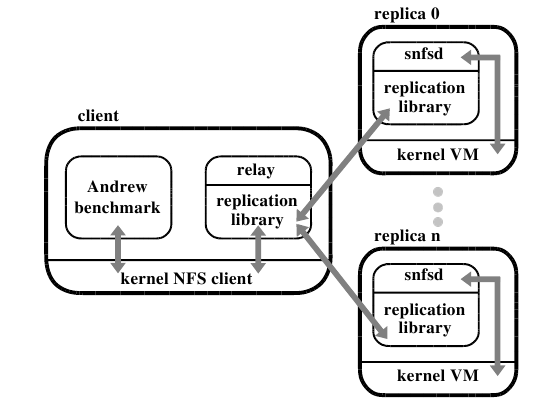
\includegraphics[width=0.8\textwidth]{nfs}
\end{figure}	
	
\end{frame}

%-------------------------------------------------------------------------
\begin{frame}{Application: Byzantine NFS server}
	
\begin{figure}
	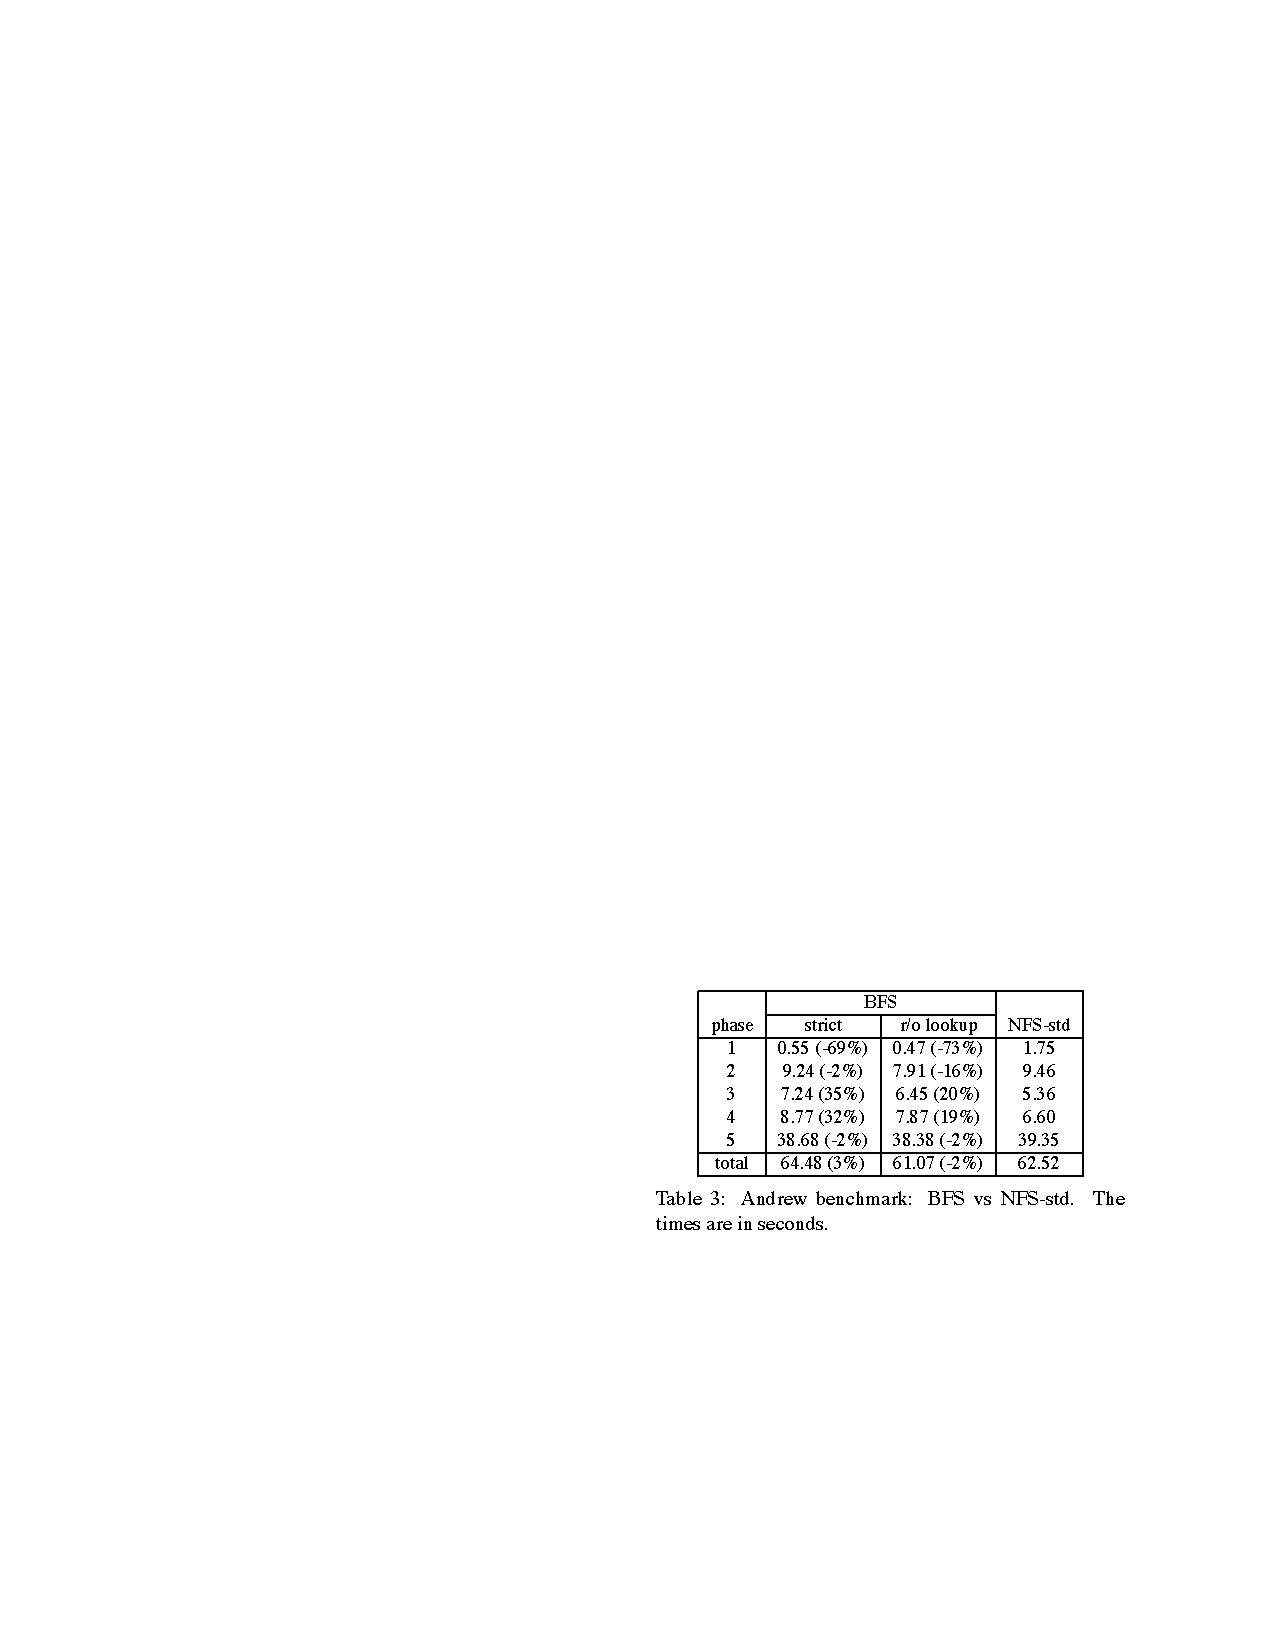
\includegraphics[width=0.8\textwidth]{andrew1}
\end{figure}	
	
\end{frame}

%-------------------------------------------------------------------------
\begin{frame}{Reality Check}
	
Example of systems that have adopted Byzantine Fault Tolerance:
\BI
\item Boeing 777 Aircraft Information Management System 
\item Boeing 777/787 flight control system
\item SpaceX Dragon flight control system
\item BitCoin
\EI
	
\end{frame}


%-------------------------------------------------------------------------
\begin{RMFrame}

\BI
\item \bibentry{pbft-osdi}
\EI

\end{RMFrame}

\end{document}